\documentclass{standalone}
\usepackage{tikz}
\usetikzlibrary{calc}

\begin{document}
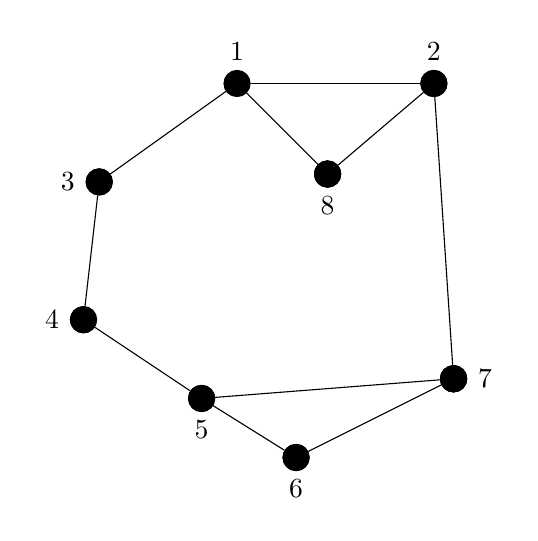
\begin{tikzpicture}[every node/.style={draw,shape=circle,fill=black}]
%Nodes
\path
 (0,0) node (p1) {}
 (2.5,0) node (p2) {}
 (-1.75,-1.25) node (p3) {}
 (-1.95,-3) node (p4) {}
 (-0.45,-4) node (p5) {}
 (0.75,-4.75) node (p6) {}
 (2.75, -3.75) node (p7) {}
 (1.15, -1.15) node (p8) {}
 ;
%Edges
\draw[-] (p1) -- (p2) node []{};
\draw[-] (p1) -- (p3) node []{};
\draw[-] (p1) -- (p8) node []{};
\draw[-] (p2) -- (p7) node []{};
\draw[-] (p2) -- (p8) node []{};
\draw[-] (p3) -- (p4) node []{};
\draw[-] (p4) -- (p5) node []{};
\draw[-] (p5) -- (p6) node []{};
\draw[-] (p6) -- (p7) node []{};
\draw[-] (p5) -- (p7) node []{};

% Adding numbers near nodes
\node[draw=none,fill=none] at ($(p1) + (0,0.4)$) {1};
\node[draw=none,fill=none] at ($(p2) + (0,0.4)$) {2};
\node[draw=none,fill=none] at ($(p3) + (-0.4,0)$) {3};
\node[draw=none,fill=none] at ($(p4) + (-0.4,0)$) {4};
\node[draw=none,fill=none] at ($(p5) + (0,-0.4)$) {5};
\node[draw=none,fill=none] at ($(p6) + (0,-0.4)$) {6};
\node[draw=none,fill=none] at ($(p7) + (0.4,0)$) {7};
\node[draw=none,fill=none] at ($(p8) + (0,-0.4)$) {8};
\end{tikzpicture}
\end{document}